\documentclass[12pt,letterpaper,english]{article}
\usepackage[utf8]{inputenc}
\usepackage[T1]{fontenc}
\usepackage[english]{babel}
\usepackage[letterpaper, margin=1in]{geometry}
\usepackage[pdftex]{graphicx}
\usepackage{fancyhdr}
\usepackage{setspace}
\usepackage{amsmath}
\usepackage{commath}
\usepackage{lastpage}
\usepackage[usenames,dvipsnames,svgnames,table]{xcolor}
\usepackage{minted}
\usepackage{isodate}
\pagestyle{fancy}
\fancyhead{}
\fancyfoot{}
\fancyhead[HR]{\thepage\ of \pageref{LastPage}}

\begin{document}


\begin{titlepage}
\thispagestyle{plain}
\begin{center}
\topskip0pt
\vspace*{\fill}

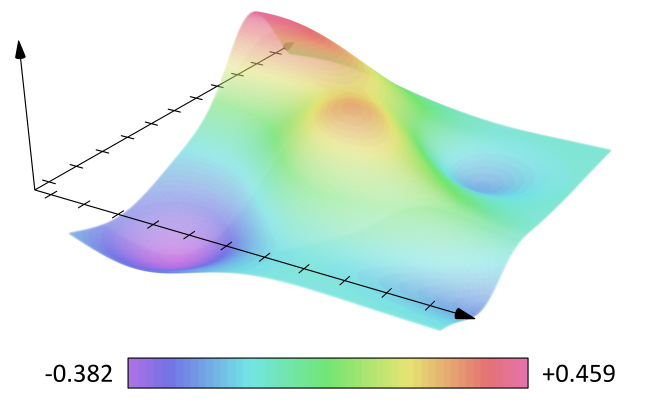
\includegraphics[width=3cm]{logo.png}~\\[1cm]

\rule{\linewidth}{0.5mm}\\[0.5cm]

\textsc{\LARGE Visualizing functions of multiple variables}\\[1cm]

\textsc{\large By Sam Grayson and Wilson Nguyen}\\[0.7cm]

{\large \isodate Version 0.1} \\[0.7cm]

\rule{\linewidth}{0.5mm}\\[1cm]

\vspace{0.9cm}

\end{center}

\section*{Abstract}

Visualizing the concepts of multivariable calculus can be challenging. The students created several computer-generated visual models utilizing the Mathematica language. These models can be used as teaching aids for educators or extra instruction for students.

\vspace*{\fill}

\end{titlepage}

\section*{Acknowledgements}

Thank you to Mrs. Harrelson for making a remarkable Multivariable Calculus class at LASA. This class is seriously the bomb if you like to think mathematically. We want to acknowledge the families of the students who have been incredibly supportive, even though they don't understand why we are doing this.

\tableofcontents

\clearpage

\doublespacing

\section{Introduction}

 As students, we know that visualizing these topics can sometimes be pretty difficult. I may or may not be guilty, on occasion, of simply using these formulas without an understanding of what they really do. If only there were some means of playing around with these topics without having to imagine clear mountains with magical rings or bleeding, toilet paper pasted shaved faces (inside joke). We believe that we have created the solution!

 The magic of Multivariable can be seen through the “Sam and Wilson’s 3D Multivariable Visualizer for Glazed-eyed LASA students” for a small fee of appreciation. The goals of this Visualizer are to allow students to interact with the topics discussed below and instead of telling the students  what the topics are, the Visualizer simply shows them. The topics would reveal themselves to even the most distant of students simply nodding their heads as asked (inside joke once more). We hope that you incorporate this Visualizer into your lessons and take advantage of the many opportunities that this opens up for students.

\section{Design Principles}

\begin{enumerate}
\item \textbf{Flexibility:} The same concept can be visualized on multiple examples, and we tried to make it so that the models can adjust at runtime to any user inputted example.
\item \textbf{Interactivity:} The concepts are best illustrated when the user can tweak the values and adjust the parameters in a dynamic way that gives real-time feedback.
\item \textbf{Maintainability:} The models \textit{look good}. They are designed to be very clean and adjustable. This means that the code may be less aligned with the mathematics, but it is worth it for ease of maintaning. This way, when we graduate the models may still be adapted to the cirriculum.
\item \textbf{Instructiveness:} The models are not by themselves. They are accompanied by text % TODO: int his paper?
explaining how they work and what they do.
\end{enumerate}




\end{document}
